\subsection{Problem 2}
\subsubsection{Interaction model}

By observing and analyzing the two images obtained from the research results of Nicky Lustenhouwer et al.\upcite{Bretschneider2011A,Lustenhouwer11551}, and using the data in the two papers related to the attachment to reproduce the images, it can be found that the hyphal extension rate is approximately in logarithmic relation with the decomposition rate, and the moisture trade-off is approximately in a linear relationship with the logarithm of the decomposition rate.

\begin{figure}[H]
    \centering
    \subfigure[]{
    \label{fig3a} 
    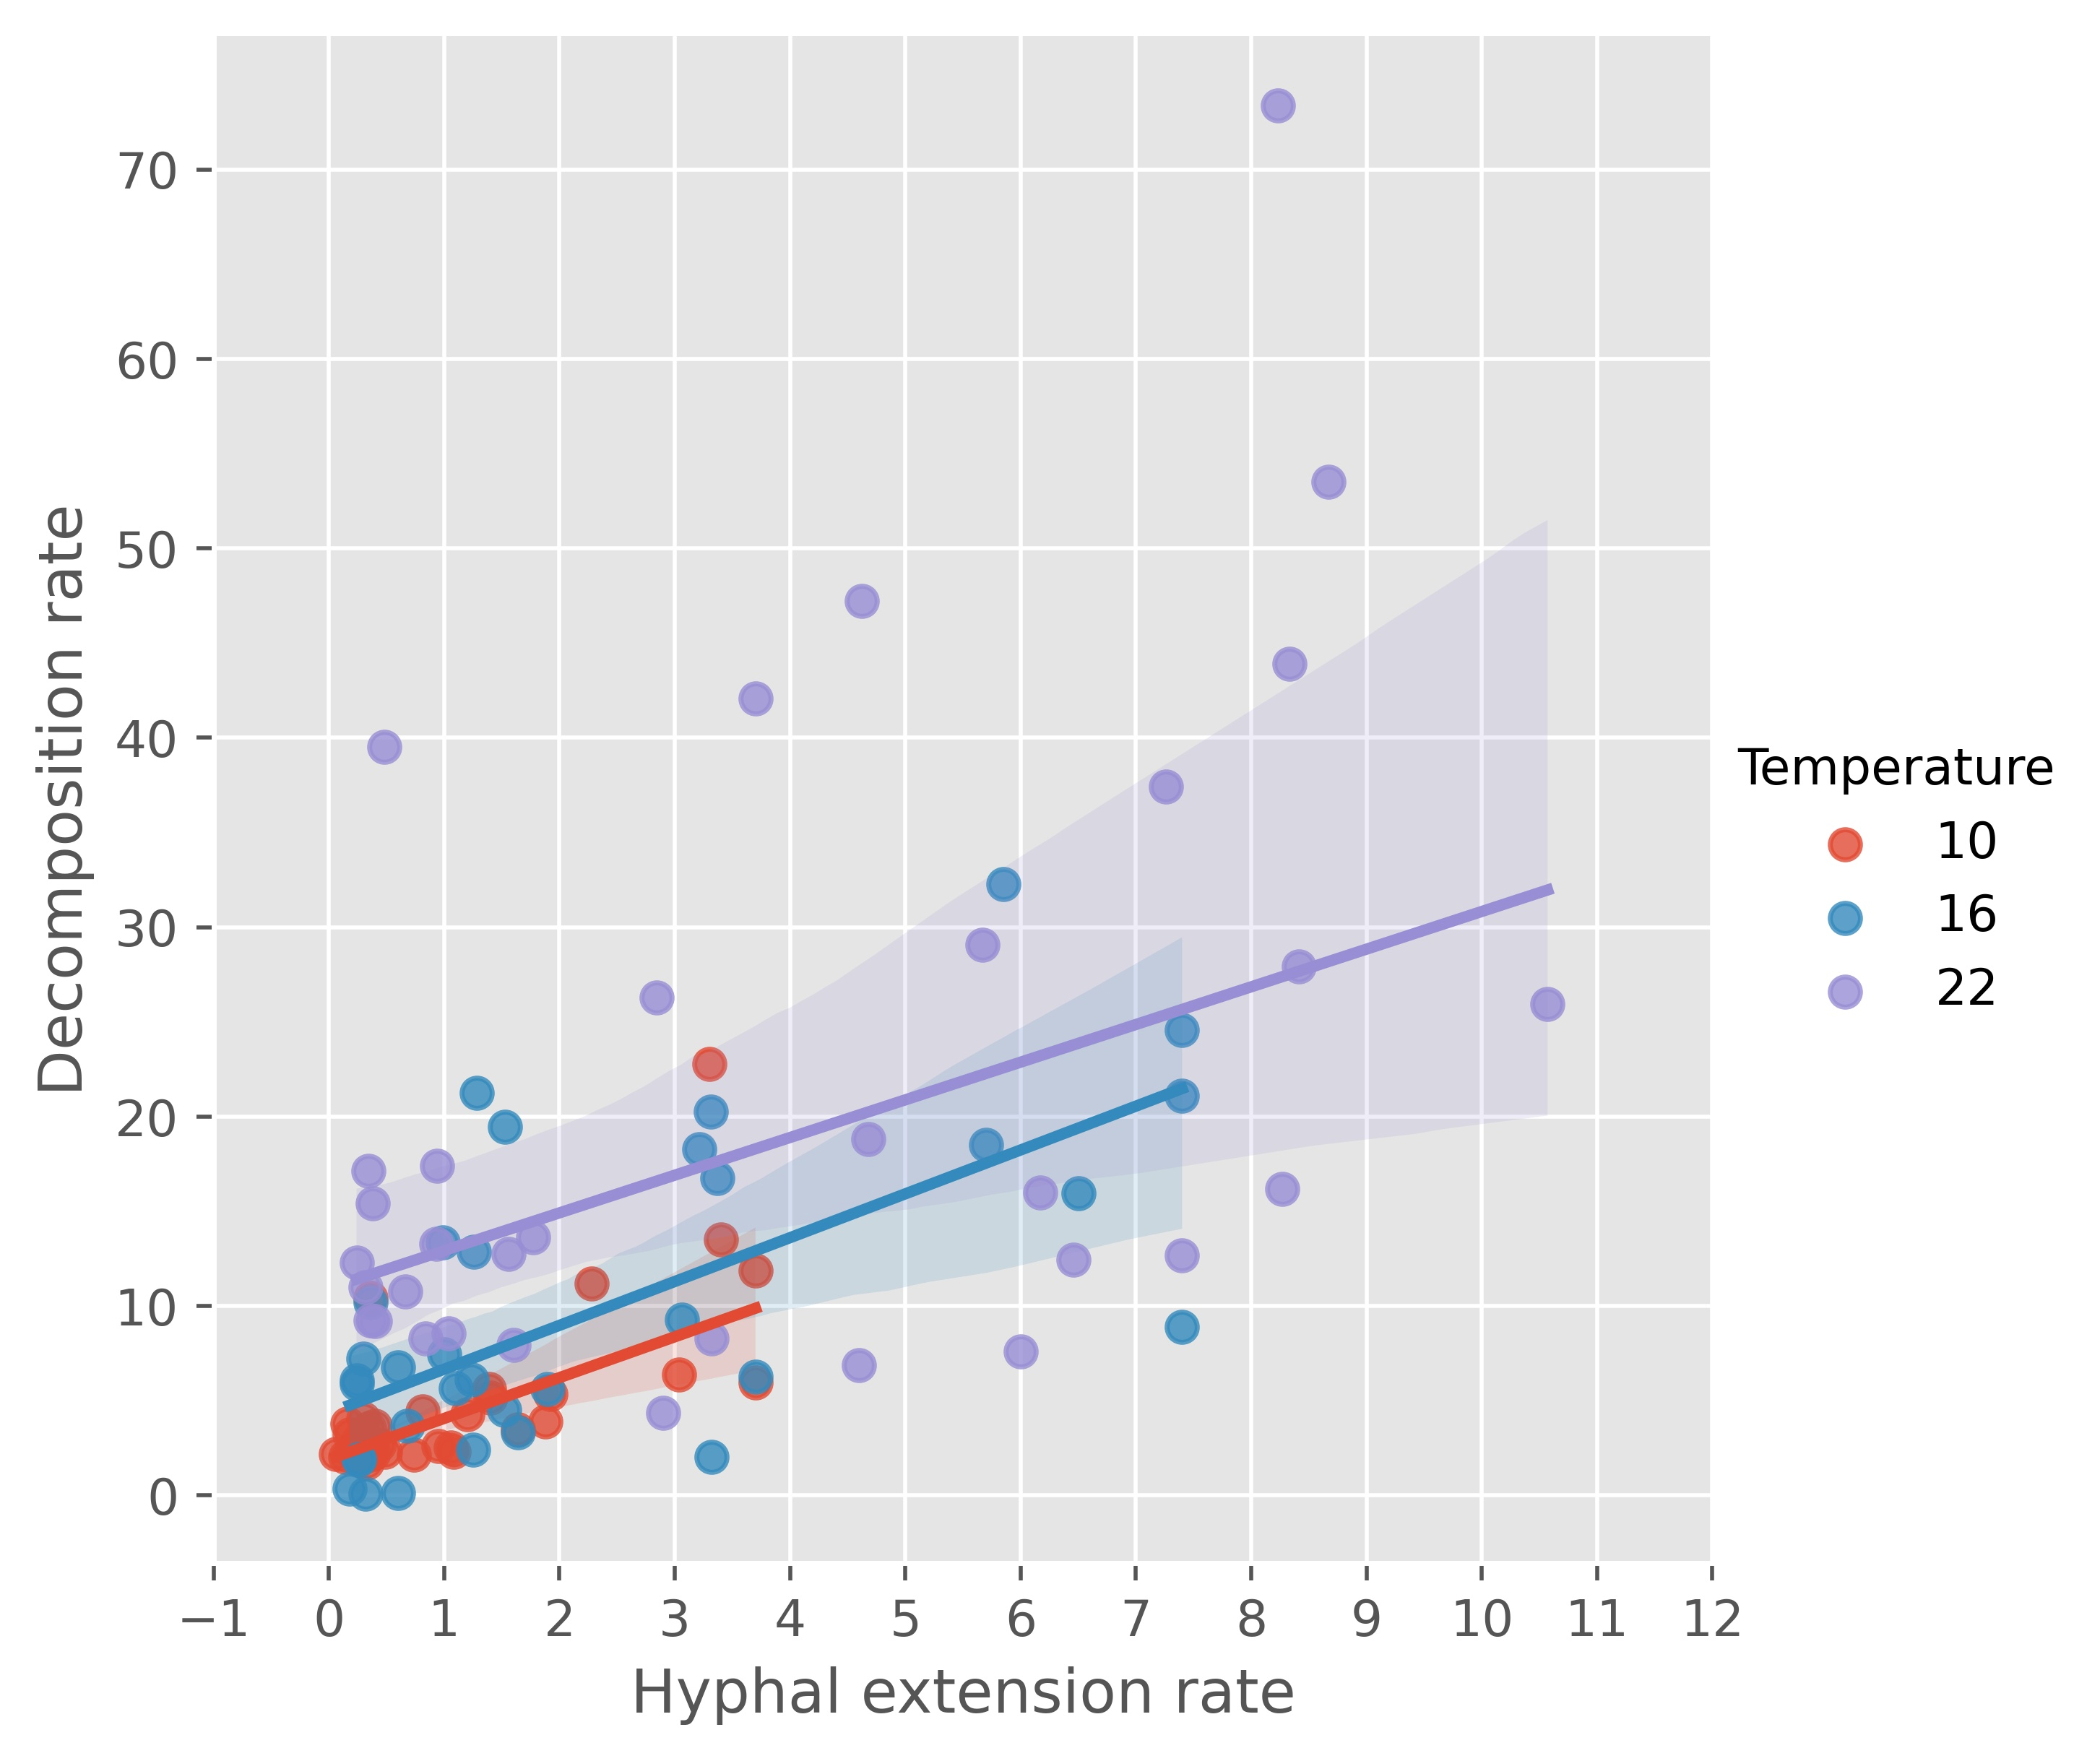
\includegraphics[scale=0.5]{./code/fig3.jpg}}
    \subfigure[]{
    \label{fig3b} 
    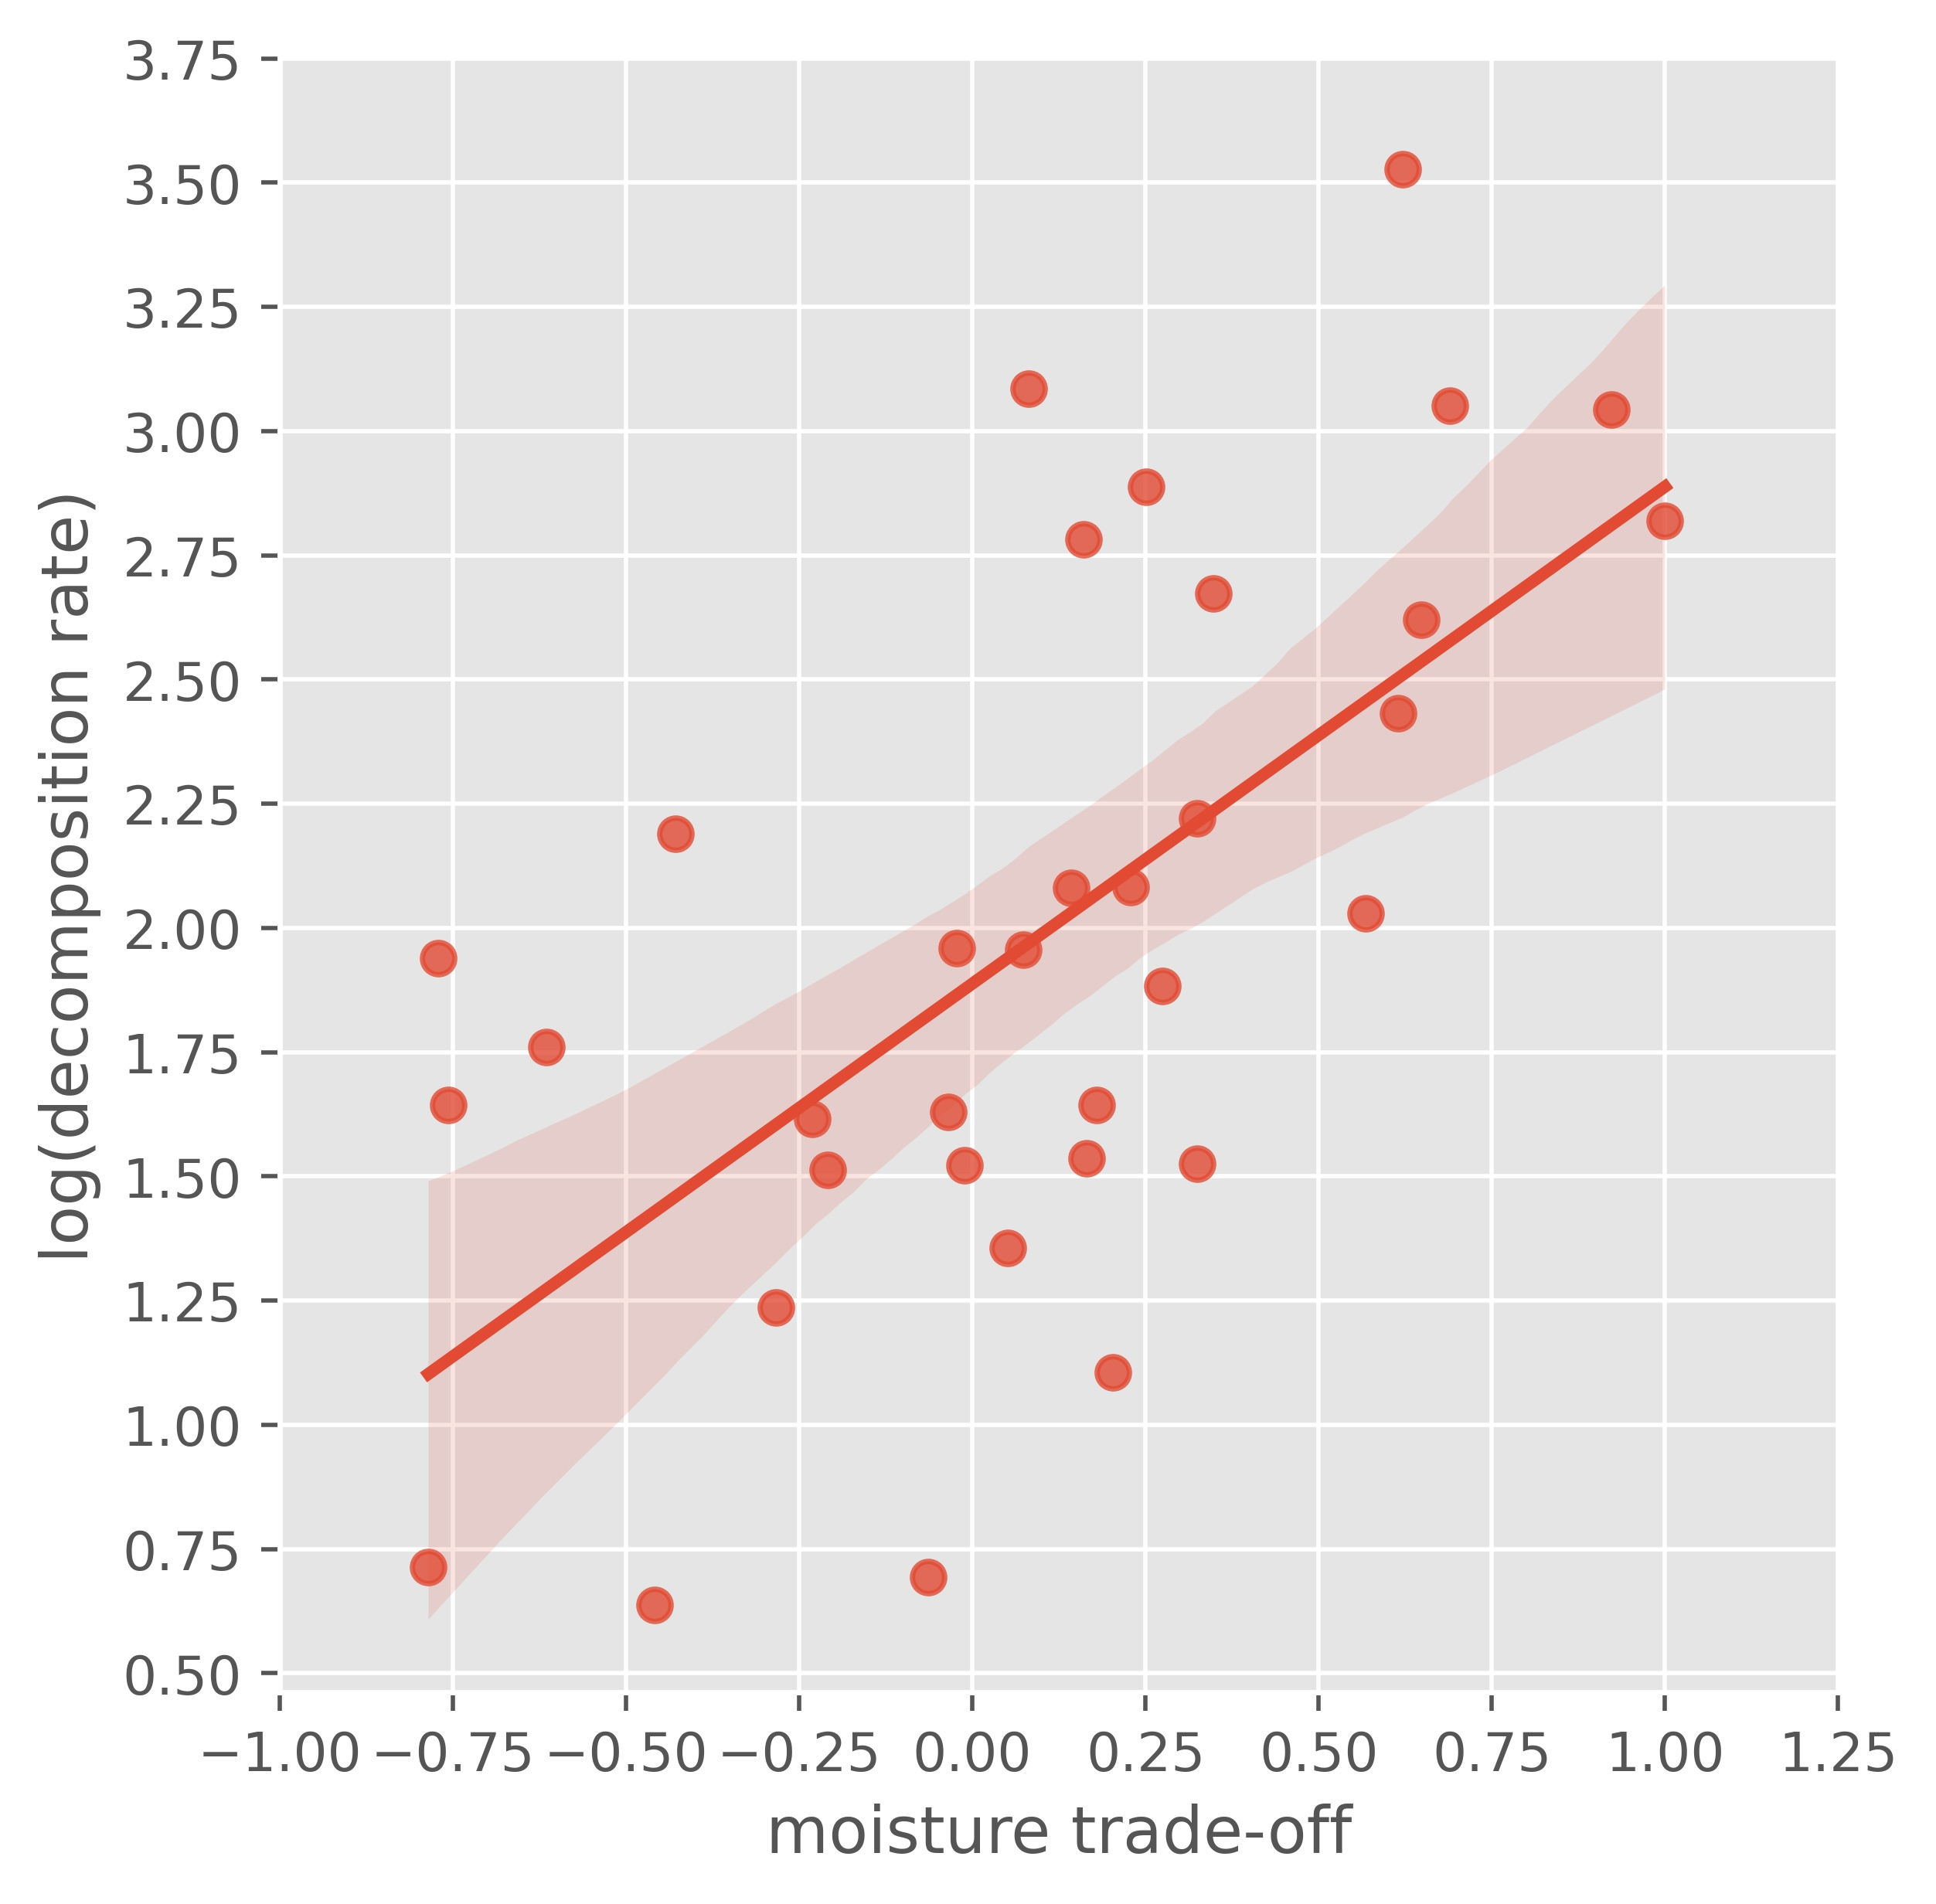
\includegraphics[scale=0.5]{./code/fig4.jpg}}
    \caption{Reproduce images from Papers}
    \label{fig3} 
\end{figure}

Therefore, assuming the decomposition rate as a constant value $Y$, the approximate relationship function between the hyphal extension rate and the decomposition rate and the approximate relationship function between the moisture trade-off and the decomposition rate can be selected as follows:
\begin{equation}\label{2.1}
    Y=a_{1}\ln{h}+b_{1}
\end{equation}
\begin{equation}\label{2.2}
    \ln{Y}=a_{2}m+b_{2}
\end{equation}

Where,

$h$ is the hyphal extension rate;

$m$ is moisture trade-off;

$a_{1}$ , $b_{1}$ , $a_{2}$ and $b_{2}$ are assumed coefficients.

After the correlation between the approximate relation function formula (\ref{2.1}) and the approximate relation function formula (\ref{2.2}), the relationship between the moisture trade-off and the hyphal extension rate can be obtained:
\begin{equation}\label{2.3}
    m=\frac{\ln{b_{1}}}{a_{1}}\ln{(a_{1}\ln{h})}-\frac{b_{2}}{a_{1}} 
\end{equation}

Then, the influences of the hyphal extension rate and moisture trade-off on decomposition rate are combined in a linear relationship, and the results are as follows:
\begin{equation}\label{2.4}
    y=am+bh+c 
\end{equation}

According to the relationship between moisture trade-off and the hyphal extension rate described in Equation (\ref{2.3}), the effects of the two factors can be combined, and then the equation (\ref{2.4}) can be converted into the expression of the decomposition rate about the hyphal extension rate:
\begin{equation}\label{}
    y=a\frac{\ln{b_{1}}}{a_{1}}\ln{(a_{1}\ln{h})}+bh+c-a\frac{b_{2}}{a_{1}} 
\end{equation}

Then simplify the above equation, and get
\begin{equation}\label{}
    y=r_{1}\ln{(r_{0}\ln{h})}+r_{2}h+r_{3}
\end{equation}

Where $r_{0},r_{1},r_{2},r_{3}$ are coefficients.

The real situation is complicated by the fact that there are many and different types of independent variables that affect the decomposition rate. In this model, linear equations are used for fitting. While simplifying the problem, the influence of various variables on the decomposition rate is also taken into consideration. And when using this model, the error of the result will decrease with the increase of data. Therefore, for the follow-up model research, our team chose to build the model with linear equations.

\subsubsection{Solution of Problem 2}

Using the above model, we can fit the relationship between decomposition rate and hyphal extension rate at different temperatures:
\begin{equation}\label{}
\left\{
\begin{array}{l}
    y=2.73x+1.855, when\ temperature = 10; (R^2=0.50)\\
    y=2.247x+4.799, when\ temperature = 16; (R^2=0.41) \\
    y=2.509x+11.48, when\ temperature = 22; (R^2=0.25) \\
\end{array}
\right.
\end{equation}
And the relationship between the decomposition rate and moisture trade-off is as follows:

\begin{equation}\label{}
    y=x+1.888; (R^2=0.40)
\end{equation}

Then, the effects of the hyphal extension rat and moisture trade-off on decomposition rate are combined with a linear relationship, and the relationship expression among the three can be obtained:
\begin{equation}\label{}
    y=0.37x_{1}+0.37x_{2}+2.07; (R^2=0.61)
\end{equation}

Where,

$x_{1}$ is the log(Hyphal extension rate)

$x_{2}$ is the moisture trade-off

$y$ is the log(decomposition rate)

The relation expression of the three is represented by Figure (\ref{4}):
\begin{figure}[H]
    \centering
    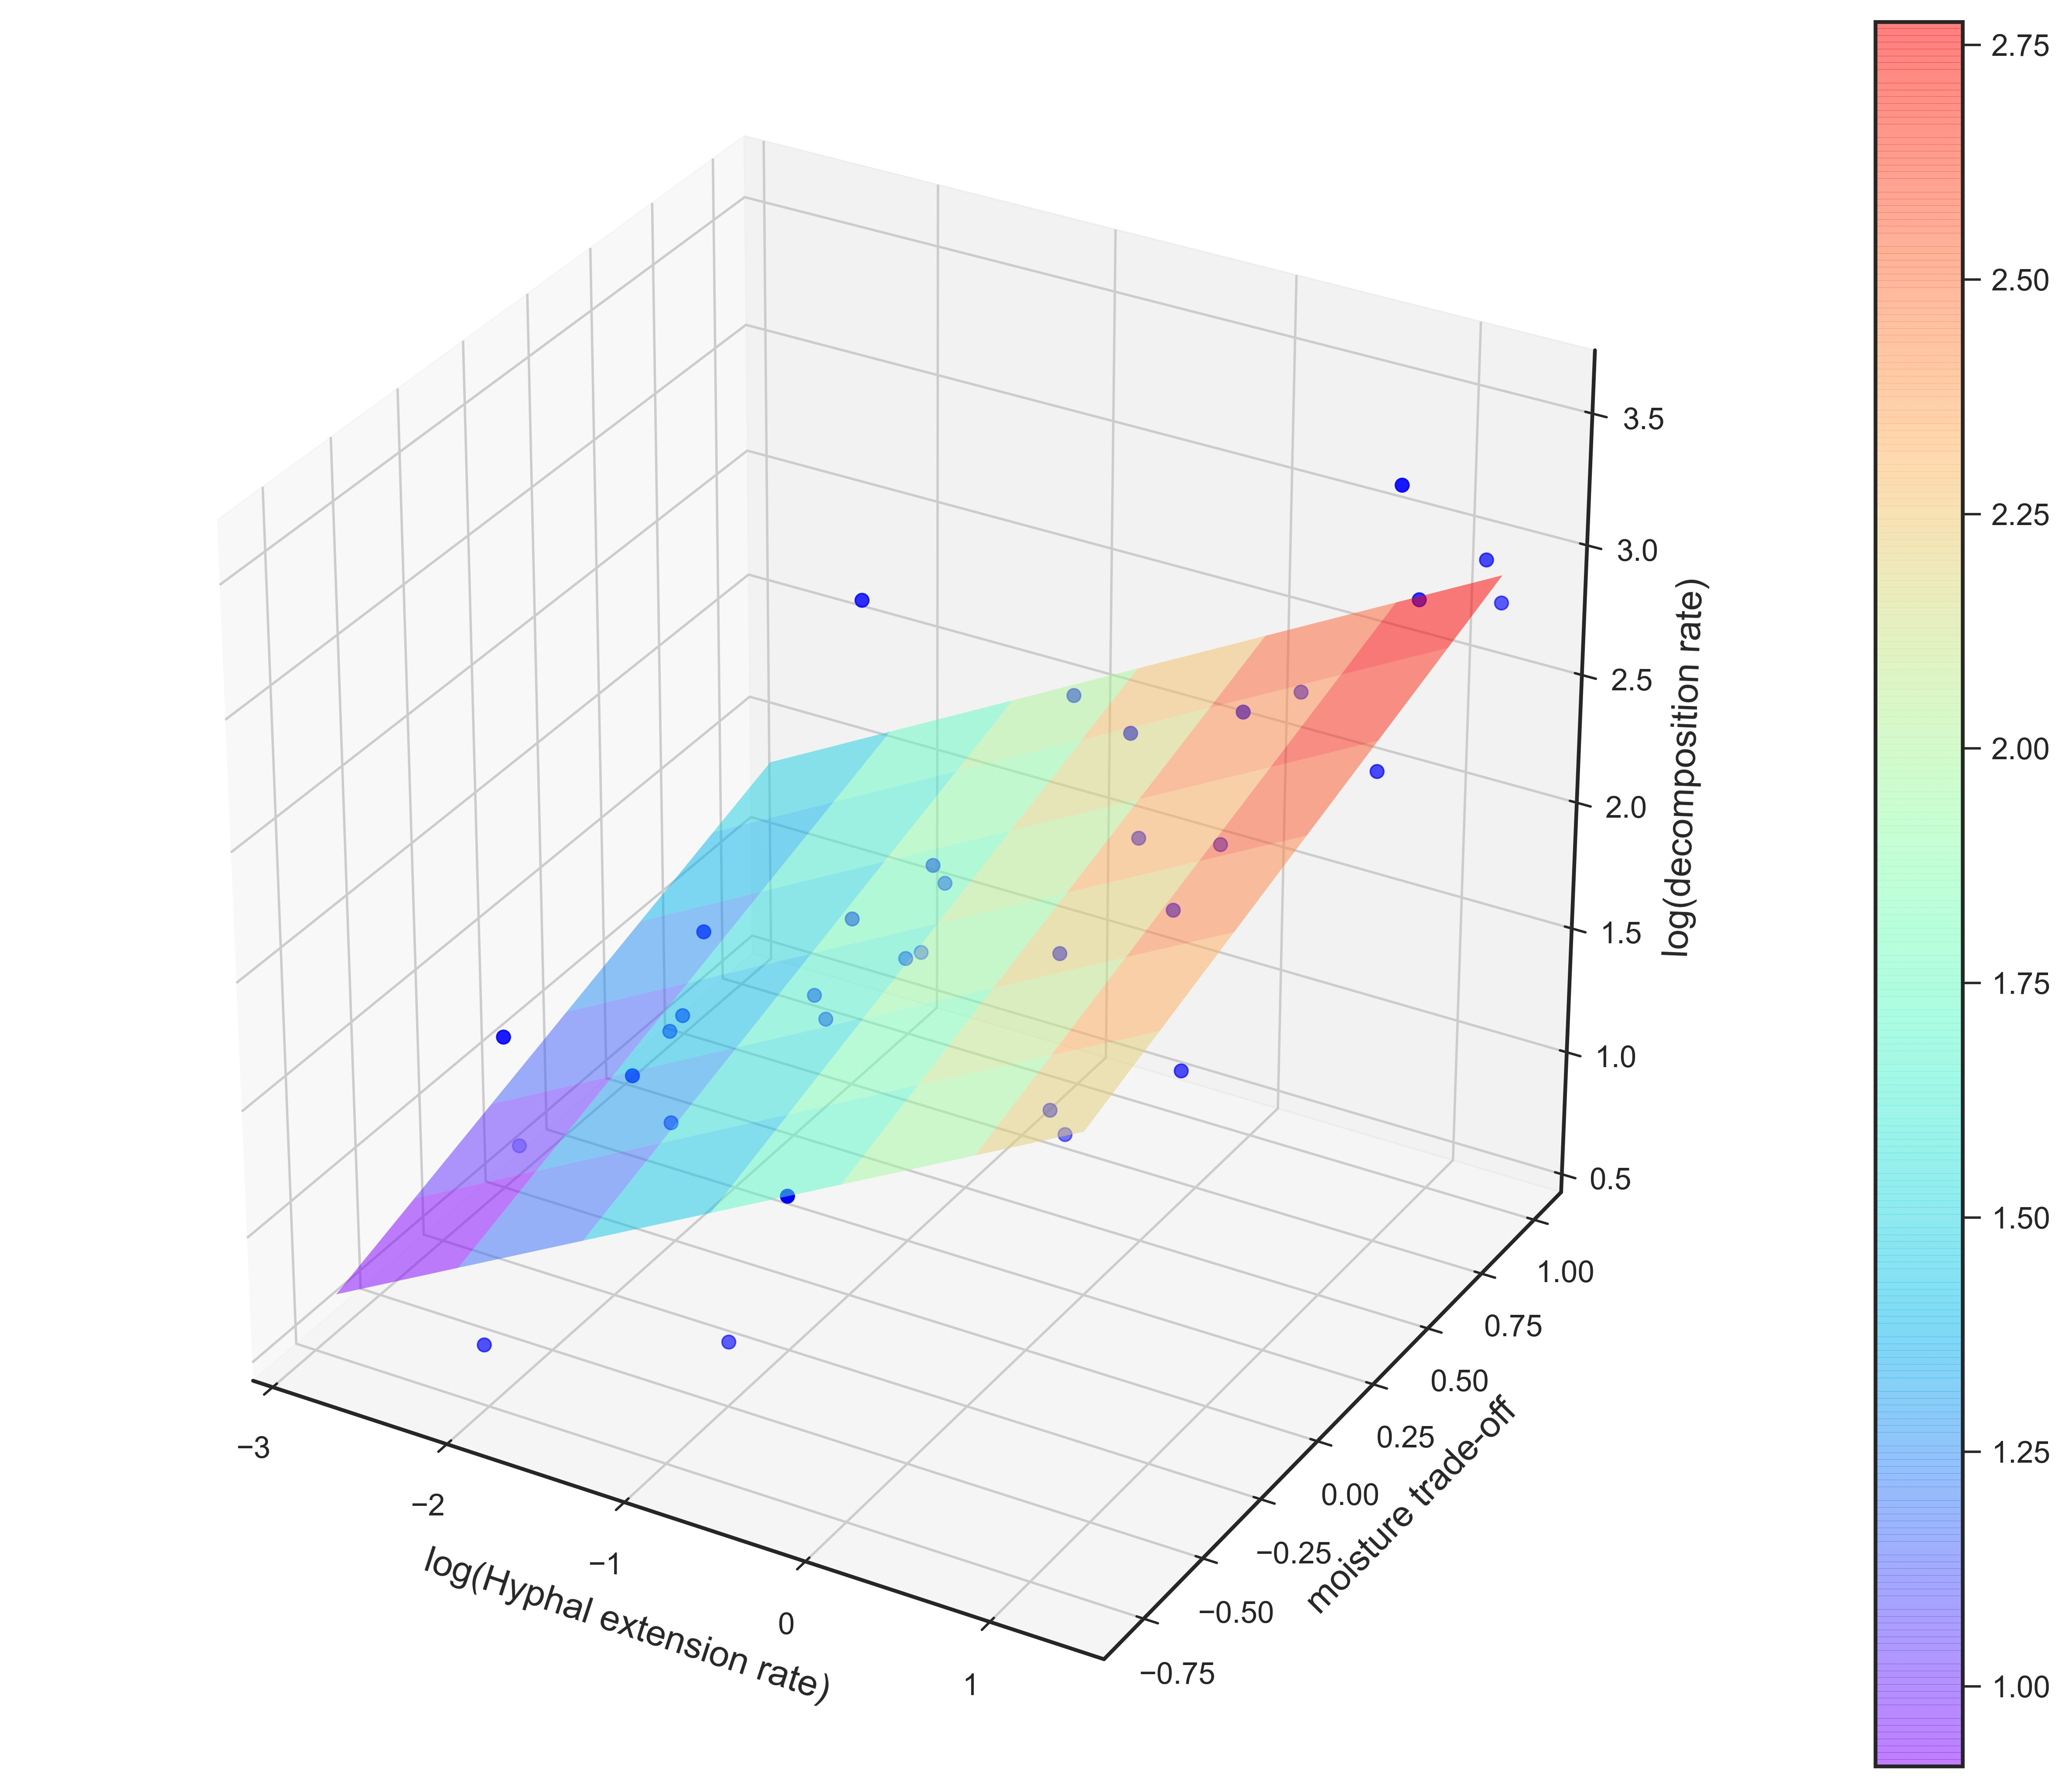
\includegraphics[width=0.8\textwidth]{./code/fig5.jpg}
    \caption{Combine hyphal extension rate and moisture trade-off on decomposition rate}\label{4}
\end{figure}

Through the fitting of the image of Decomposition rate -- Hyphal extension rate, we find that the fitting effect with "logarithmic relationship" is far less good than that with "linear relationship". Therefore, Equations (\ref{2.1}) and (\ref{2.3}) are improved to Equations (\ref{2.1*}) and (\ref{2.3*}).
\begin{equation}\label{2.1*}
    Y=a_{1}h+b_{1}
\end{equation}
\begin{equation}\label{2.3*}
    m=\frac{\ln{b_{1}}}{a_{1}}\ln{(a_{1}h)}-\frac{b_{2}}{a_{1}} 
\end{equation}

After combining Hyphal Extension Rate and Moisture Trade-Off, the following formula can be obtained:
\begin{equation}\label{2.5}
    y=r_{1}\ln(r_{0}h)+r_{2}h+r_{3}
\end{equation}

The results obtained by this method accord with the expected effect and the error is small.